\documentclass[9pt]{pnas-new}
% Use the lineno option to display guide line numbers if required.
% Note that the use of elements such as single-column equations
% may affect the guide line number alignment. 

%\RequirePackage[english,slovene]{babel} % when writing in slovene
\RequirePackage[slovene,english]{babel} % when writing in english

%\templatetype{pnasresearcharticle} % Choose template 
\templatetype{pnasresearcharticle} % = Template for a two-column research article
% {pnasmathematics} = Template for a one-column mathematics article
% {pnasinvited} = Template for a PNAS invited submission

\usepackage{subcaption}
\usepackage{graphicx}
\usepackage{float}

%\selectlanguage{slovene}
%\etal{in sod.} % comment out when writing in english
%\renewcommand{\Authands}{ in } % comment out when writing in english
%\renewcommand{\Authand}{ in } % comment out when writing in english

\newcommand{\set}[1]{\ensuremath{\mathbf{#1}}}
\renewcommand{\vec}[1]{\ensuremath{\mathbf{#1}}}
\newcommand{\uvec}[1]{\ensuremath{\hat{\vec{#1}}}}
\newcommand{\const}[1]{{\ensuremath{\kappa_\mathrm{#1}}}} 

% Custom commands for Easier writing
\renewcommand{\etal}{et al.\ }
\newcommand{\eg}{e.g., }
\newcommand{\ie}{i.e., }
\newcommand{\wrt}{w.r.t. }
\newcommand{\etc}{etc.}
\newcommand{\na}{\emph{n.a.} }

\newcommand{\num}[1]{#1}

\title{Simulating Coral Competition and Growth in a 3D Environment}

% Use letters for affiliations, numbers to show equal authorship (if applicable) and to indicate the corresponding author
\author{Nejc Hirci}

\affil{Collective behavior course research seminar report} 

% Please give the surname of the lead author for the running footer
\leadauthor{Hirci} 

\selectlanguage{english}

% Please add here a significance statement to explain the relevance of your work
\significancestatement{Significance Statements}{
Understanding coral competition and growth dynamics is vital for effective restoration in response to climate-induced threats to coral reefs. Inspired by Cresswell \etal~\cite{coral_community_3D}, we implement space colonization growth principles in their proposed model, capturing diverse ecological processes.
}


% Please include corresponding author, author contribution and author declaration information
\authorcontributions{Please provide details of author contributions here.}
\authordeclaration{Please declare any conflict of interest here.}
\equalauthors{\textsuperscript{1}A.O.(Author One) and A.T. (Author Two) contributed equally to this work (remove if not applicable).}
\correspondingauthor{\textsuperscript{2}To whom correspondence should be addressed. E-mail: author.two\@email.com}

% Keywords are not mandatory, but authors are strongly encouraged to provide them. If provided, please include two to five keywords, separated by the pipe symbol, e.g:
\keywords{Coral simulation, collective behavior, procedural modeling} 

\begin{abstract}

This article introduces a new extension to coral simulation models, merging a three-dimensional cellular automata growth model with a complex model of coral growth. In response to climate-induced threats to coral reefs, understanding coral competition and growth dynamics is vital for effective restoration. Inspired by Cresswell \etal~\cite{coral_community_3D}, we implement space colonization growth principles in their proposed model, capturing diverse ecological processes. The real-time simulation of the model is developed as a web-application available at \url{https://nejchirci.github.io/CoralSimulation}. This research contributes a visually compelling real-time simulation model, enhancing our understanding of coral community dynamics and offering insights for reef restoration and conservation in the face of environmental challenges.
\end{abstract}

\dates{\textbf{\today}}
\program{BM-RI}
\vol{2023/24}
\no{CB:G1} % group ID
\fraca{FRIteza/201516.130}

\begin{document}

% Optional adjustment to line up main text (after abstract) of first page with line numbers, when using both lineno and twocolumn options.
% You should only change this length when you've finalised the article contents.
\verticaladjustment{-2pt}

\maketitle
\thispagestyle{firststyle}
\ifthenelse{\boolean{shortarticle}}{\ifthenelse{\boolean{singlecolumn}}{\abscontentformatted}{\abscontent}}{}

\section*{Introduction}

In marine biology, coral reefs have been an essential research subject for many years due to their importance in preserving marine wildlife and their naturally high biodiversity. Unfortunately, they are also one of the ecosystems most susceptible to the various environmental changes brought about by climate change. Much of current marine research focuses on the restoration efforts of coral reefs, for which it is crucial to understand the environmental factors that affect coral communities. For such purposes, we need ways to adequately simulate many complicated ecological processes in four dimensions. Much existing research focuses on empirically tested models, which provide essential simulation output variables (\eg coral communities coverage) but are often limited to two dimensions. We provide a real-time implementation of an existing three-dimensional~\cite{coral_community_3D} coral reef model with some extensions to the coral growth simulation.

\section*{Related Work}

Most models that focus on analyzing the behavior of coral reefs limit themselves to a two-dimensional setting because introducing another spatial dimension requires a considerably more complex growth model. They form a theoretical baseline for some of the more recent three-dimensional models~\cite{coral_community_3D}.

One of the recent review studies by Weijerman \etal~\cite{coral_models_review} describes a precise categorization of ecological model design approaches based on their leading principles. One of the major leading principles is to design models suited for extrapolation and long-term projections of coral community dynamics. These require complex sub-models of various ecological processes and often rely on prior research to achieve realistic long-term predictions.

Agent-based approaches are most commonly used to explore coral competition under changing conditions. They are well suited to introduce coral-community dynamics based on diversity, functional individual traits, and demography of a coral reef, and can be used with submodels of varying complexity. This is seen in a recently developed model by Carturan \etal~\cite{coral_community_main}, extended with trait-based approaches from existing databases. Their model shows an extensive set of simulated ecological processes (bleaching, reproduction, sedimentation, algae invasion, \etc) and includes a set of 798 functionally realistic species defined using 11 functional traits carefully designed from empirical data.

Turning our attention to three-dimensional simulation models, one of the recent papers by Cresswell \etal~\cite{coral_community_3D} describes a three-dimensional functional-structural model, \textit{Coralcraft}, focused on investigating the influence of hydrodynamic disturbances on coral communities. They simulate five different coral morphologies: encrusting, hemispherical, tabular, corymbose, and branching, with a three-dimensional cell grid. Light, shading, nutrient distribution, and hydrodynamic disturbances all influence the growth of each polyp. They cover major ecological processes, growth, recruitment, and mortality but lack some minor ones, like algae invasions, bleaching, and dislodgement. Nevertheless, they provide a reliable baseline we use in our work.

While there have been only few three-dimensional simulation models, we can find several three-dimensional growth models that provide somewhat realistic results. They provide general models of either stone or soft corals, because of significant differences between them. The former form hard external calcium carbonate skeletons, while the latter are held together by jelly-like mesoglea and internal rigid structures~\cite{corals_book_1983}. Merks \etal~\cite{polyp_growth} were one of the first to address growth on a polyp-level scale. Their performs voxelization to polyps, resource transport in the environment, and the accretion step of actual growth on each mesh vertex. Kaandorp \etal~\cite{Kaandorp_2013} later extended their work by introducing a fluid flow model and an extension of the dispersion of nutrients by advection-diffusion. Recent work by O'Hagan \etal~\cite{sponge_growth} noted that their accretive growth model may only partially fit to simulate the coral growth of sponges. 

We found the accretive growth model to be too complex, to be integrated on top of the existing \textit{Coralcraft} model. We use a less performance, intensive method based on the space colonization algorithm. In its most recent form it was described by Runions~\etal~\cite{space_colonization_3d} specifically for generating realistic tree structures. It works by growing a skeleton from the root node towards the nearest points of attraction, which represent the distributed nutrients in our case. We introduce some minor modifications, to utilize this approach in generating the branching and corymbose corals, which more closely resemble tree canopies.

\section*{Methods}

The \textit{Coralcraft} model demonstrates the impact of hydrodynamic disturbances on coral communities. It uses $1cm^3$ voxels to represent the lowest spatial level of computation, equivalent to one coral colony polyp. The model integrates sub-modules of the main ecological processes of growth, reproduction, mortality, and hydrodynamic disturbance. It describes five functional morphologies: branching, tabular, encrusting, hemispherical, and corymbose corals, as shown in Figure~\ref{fig:morphologies}.

\begin{figure}[H]
    \centering
    \begin{subfigure}{0.12\textwidth}
        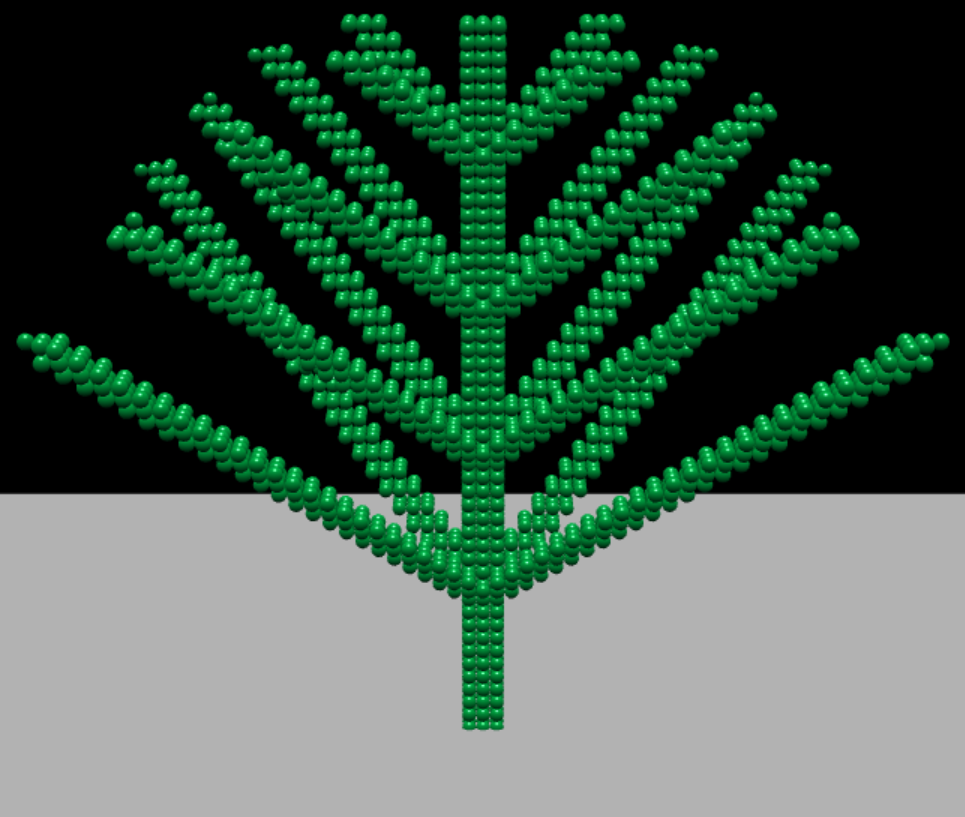
\includegraphics[width=\textwidth]{fig/branching.png}
    \end{subfigure}
    \begin{subfigure}{0.12\textwidth}
        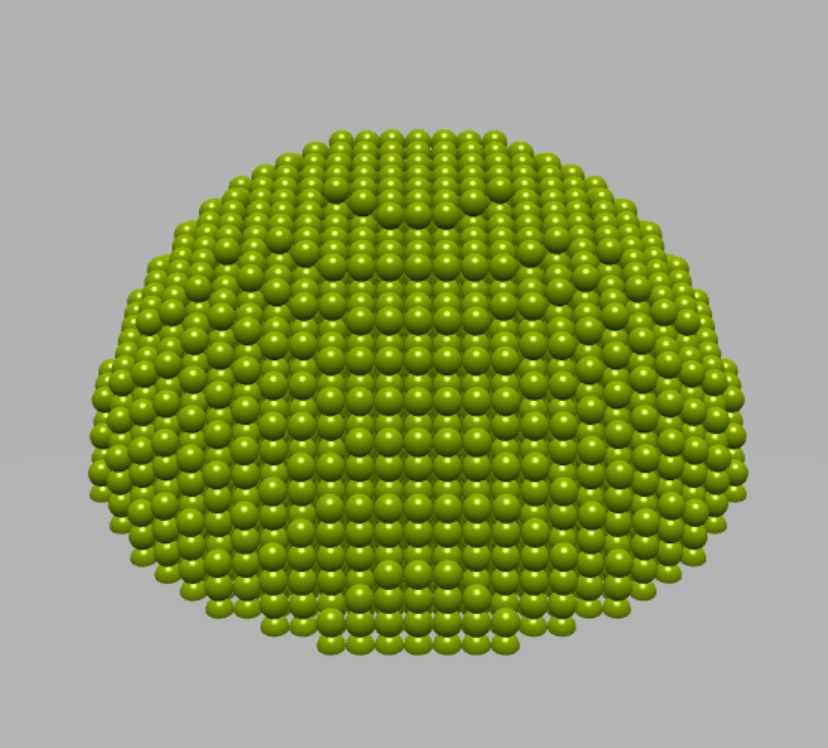
\includegraphics[width=\textwidth]{fig/hemispherical.png}
    \end{subfigure}
    \begin{subfigure}{0.12\textwidth}
        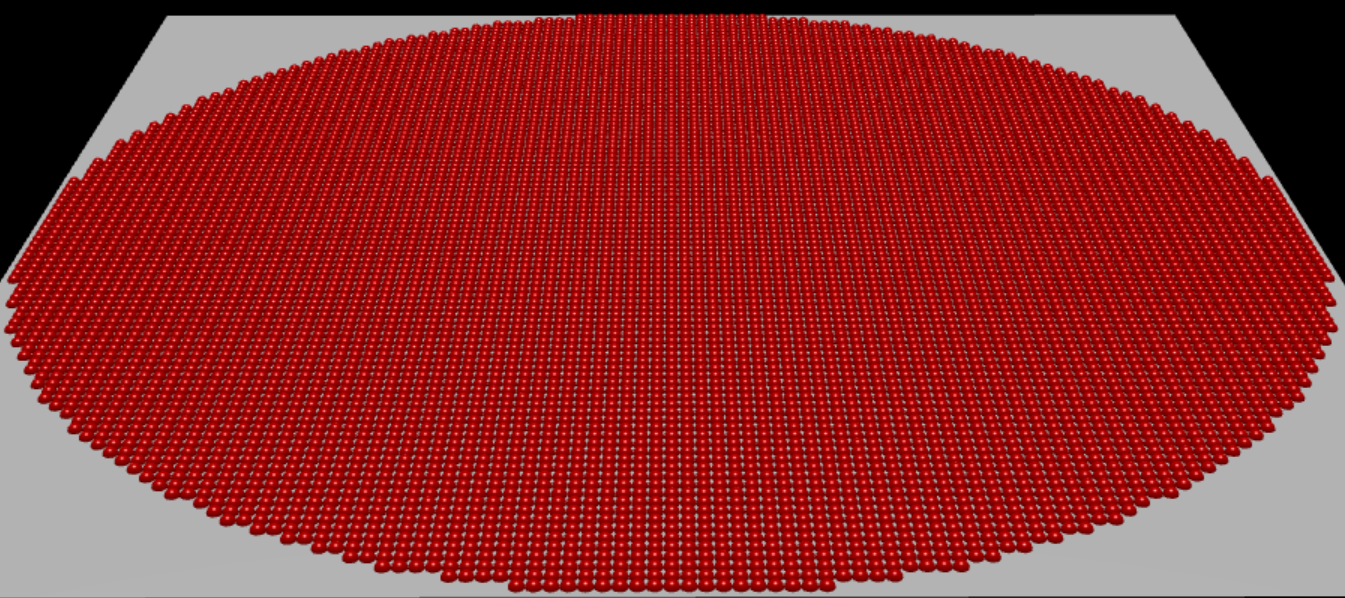
\includegraphics[width=\textwidth]{fig/encrusting.png}
    \end{subfigure}
    \begin{subfigure}{0.12\textwidth}
        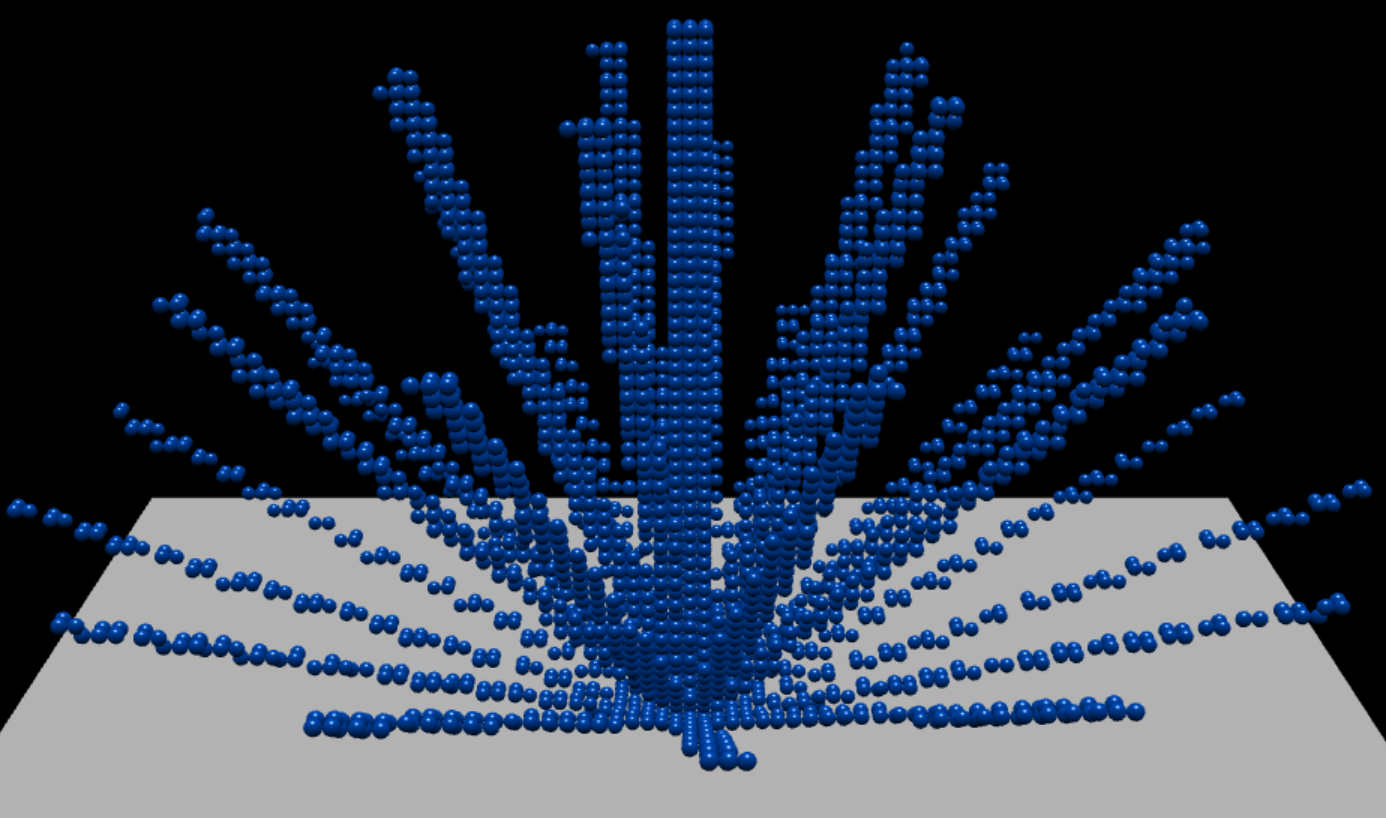
\includegraphics[width=\textwidth]{fig/corymbose.png}
    \end{subfigure}
    \begin{subfigure}{0.12\textwidth}
        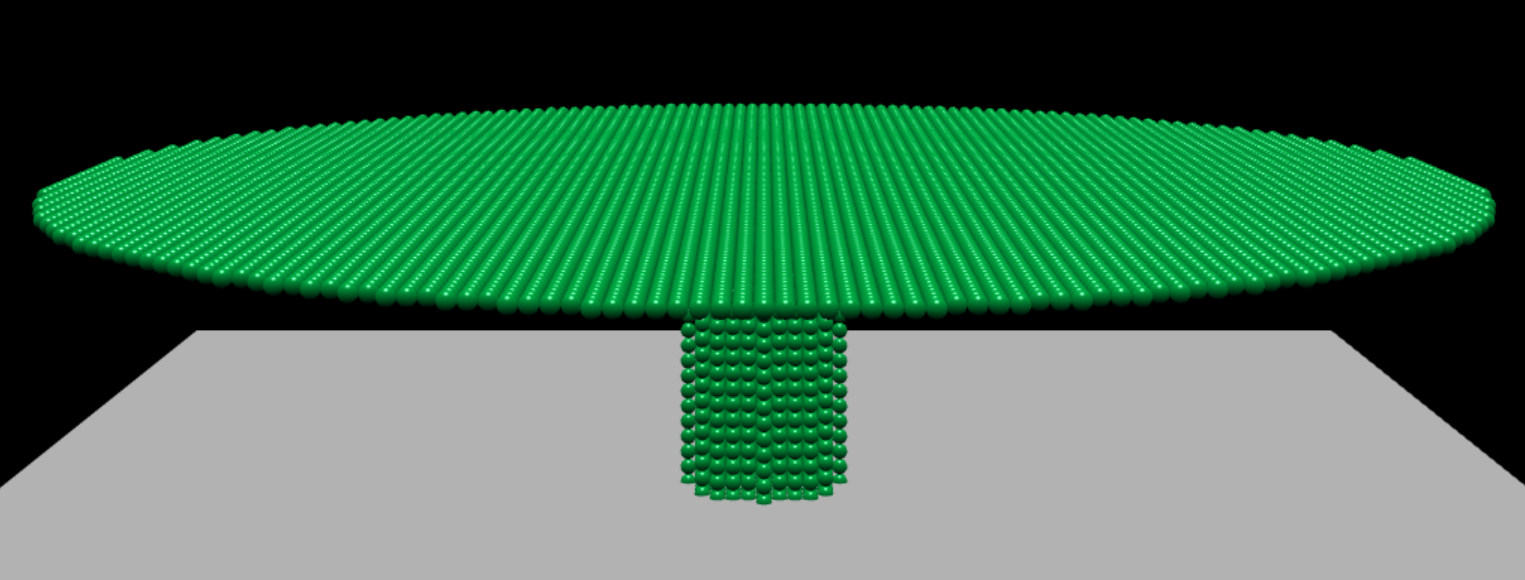
\includegraphics[width=\textwidth]{fig/tabular.png}
    \end{subfigure}
    \caption{Five coral morphologies (left to right): Branching, Hemispherical, Encrusting, Corymbose, Tabular.}
    \label{fig:morphologies}
\end{figure}

The simulation steps are presented in Figure~\ref{fig:base_model} and consist of the initial placement of colonies; light attenuation and nutrient distribution; growth and dead of corals according to the amount of received resources.

\begin{figure}[H]
    \centering
    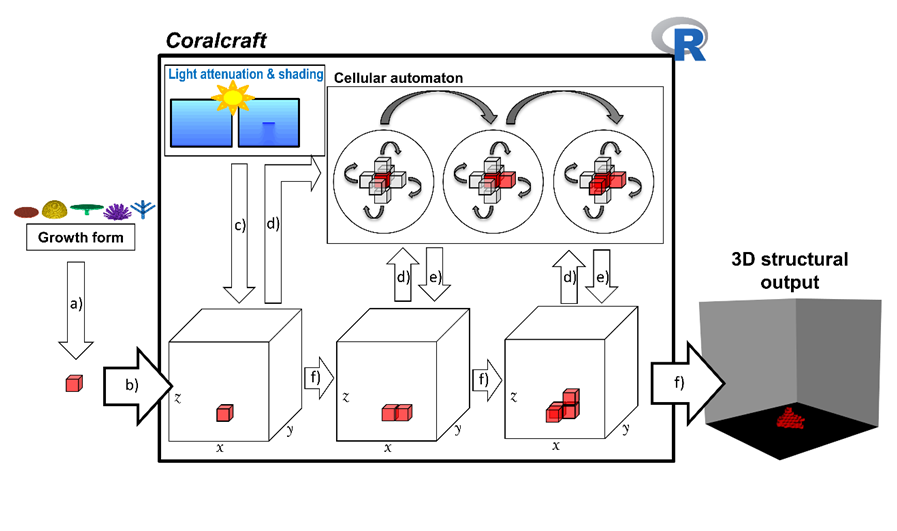
\includegraphics[width=0.5\textwidth]{fig/model.png}
    \caption{The baseline \textit{Coralcraft} model~\cite{coral_community_3D}.}
    \label{fig:base_model}
\end{figure}

The most expensive step in the simulation is the computation of light attenuation. It is calculated at each vertical layer of the cellular grid, where 99.67\% of light is passed to voxels in the layer below (based on the Beer-Lambert-Bouguer law). To account for shading, 50\% of light travels directly downwards and the other 50\% is equally distributed among neighboring voxels.

Additionally, the simulation includes the processes of reproduction, sedimentation, natural mortality, and hydrodynamic disturbance with specified frequencies. Reproduction is simulated as a random occupation of voxels on the seafloor (y==0) once every year, where we choose the morphologies of recruits according to the number of cells belonging to each morphology.

Hydrodynamic disturbances are integrated by computing the colony shape factor (CSF), a dimensionless index of mechanical vulnerability to horizontal forces. The formula considers the side profile of the colony along with the size of the basal attachment to the sea floor,

\begin{equation*}
    \text{CSF} = \frac{16}{d_{\text{profile}}^2d_{\text{basal}}} \int_{y=0}^h y w(y) dy
\end{equation*}

where $d_{\text{profile}}$ $d_{\text{basal}}$ are measured to be the number of voxels parallel and perpendicular, to a horizontal wave motion. Higher shape factor means poorer structural robustness.

We extend the growth ob branching and corymbose corals with the space colonization algorithm, to more closely resemble real-life corals. We do not use it for tabular, encrusting, and brain corals, which do not exhibit strong branching behaviors. The space colonization works by procedurally growing the branches of the coral from the root polyp in the directions of the nutrient distributions, but still in accordance with the overall shape specified by the \textit{Coralcraft} model. This yields greater variation and more realistic results than the initial model.

We validate our model by observing simulation outputs of flat percentage cover, volume percentage cover, linear rugosity, and diversity of the model. Linear rugosity is an important indicator of the overall robustness of the reef, as well as the abundance of marine life and species. It describes the structural complexity of the reef, calculated as the ratio of the distance required to cover a fixed flat distance when traversing coral communities. The diversity of the simulation is computed using Simpson’s Diversity Index, 

\begin{equation}
    \text{SDI} = 1 - \sum (\frac{n}{N})^2
\end{equation}

where $n$ is the number of individuals displaying a specific morphology and $N$ is the total number of individuals. In our case with 5 morphological types, the highest possible diversity is 0.8.

We developed a web application using established web development technologies, such as Node.js~\cite{nodejs} and the Typescript programming language, and the Babylon.js~\cite{babylonjs} library for rendering the scene. We also include a user interface, which offers control over different simulation parameters, tracking of simulation events, and visualizing the output variables. 

\section*{Results}

We simulate 10 years of coral growth under different levels of hydrodynamic disturbance. First, we use the estimated fixed frequency of disturbances as used in the \textit{Coralcraft} research paper, that is every two years varying between low and high intensities. The Figure~\ref{fig:moderate}, shows that encrusting and hemispherical corals start to dominate the reef very soon, and while the rugosity of the model, does slowly increase, the diversity drops significantly.

\begin{figure}[H]
    \centering
    \begin{subfigure}{0.35\textwidth}
        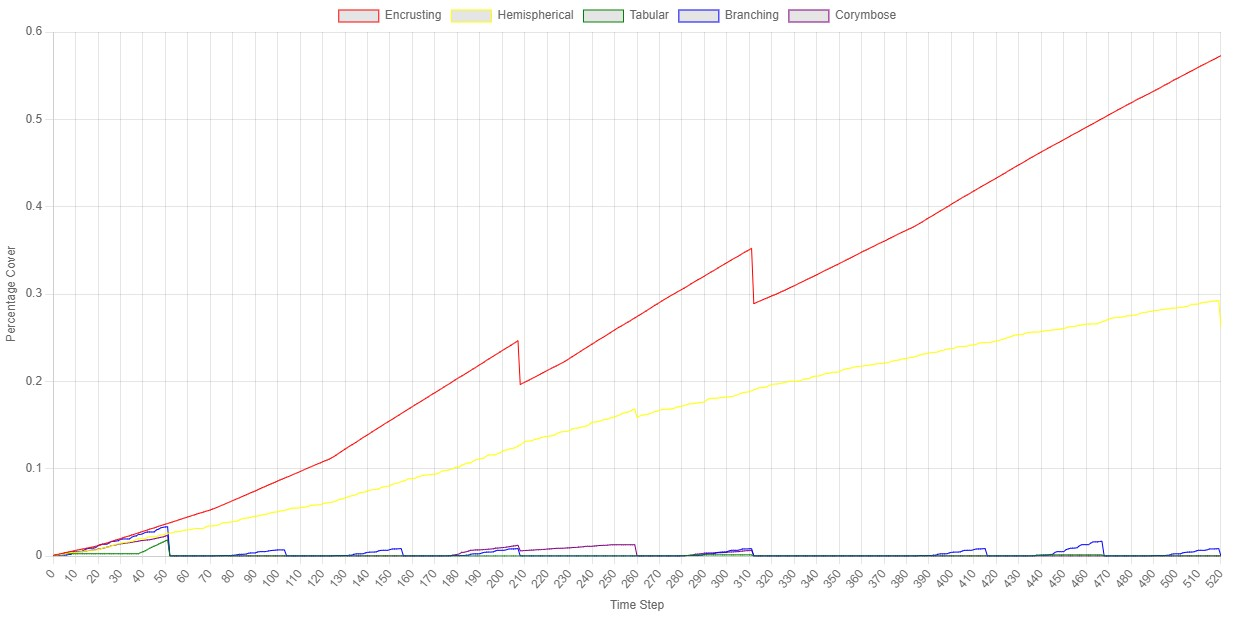
\includegraphics[width=\textwidth]{fig/moderate_chart_cover.jpg}
    \end{subfigure}
        \begin{subfigure}{0.35\textwidth}
        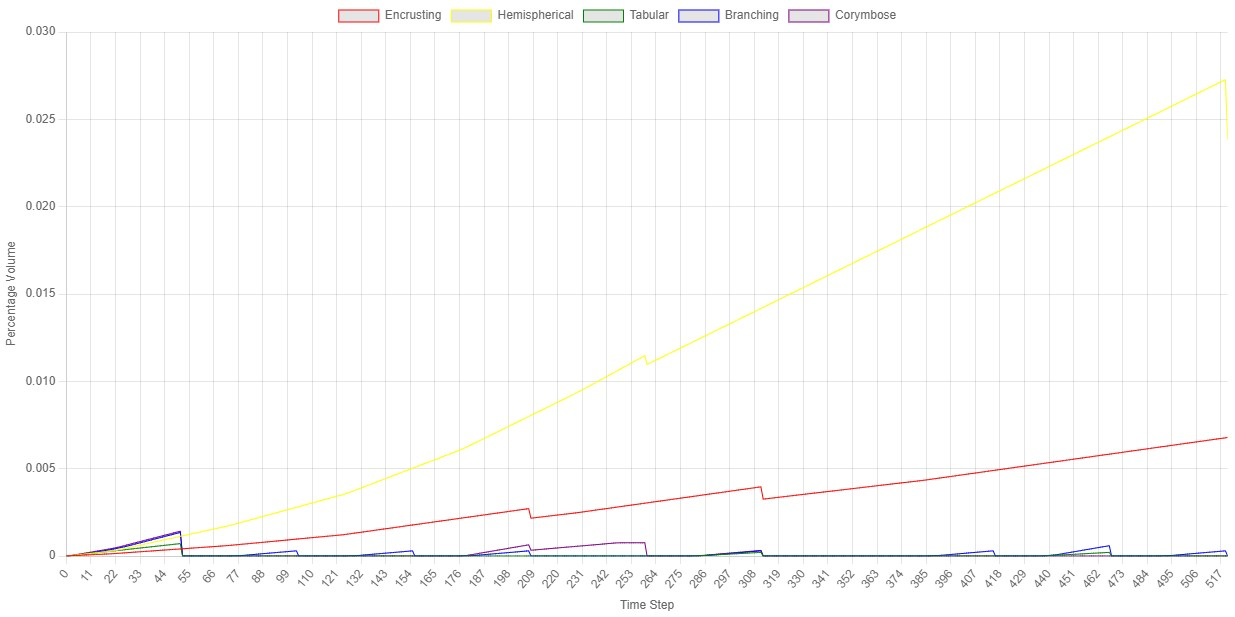
\includegraphics[width=\textwidth]{fig/moderate_chart_volume.jpg}
    \end{subfigure}
        \begin{subfigure}{0.35\textwidth}
        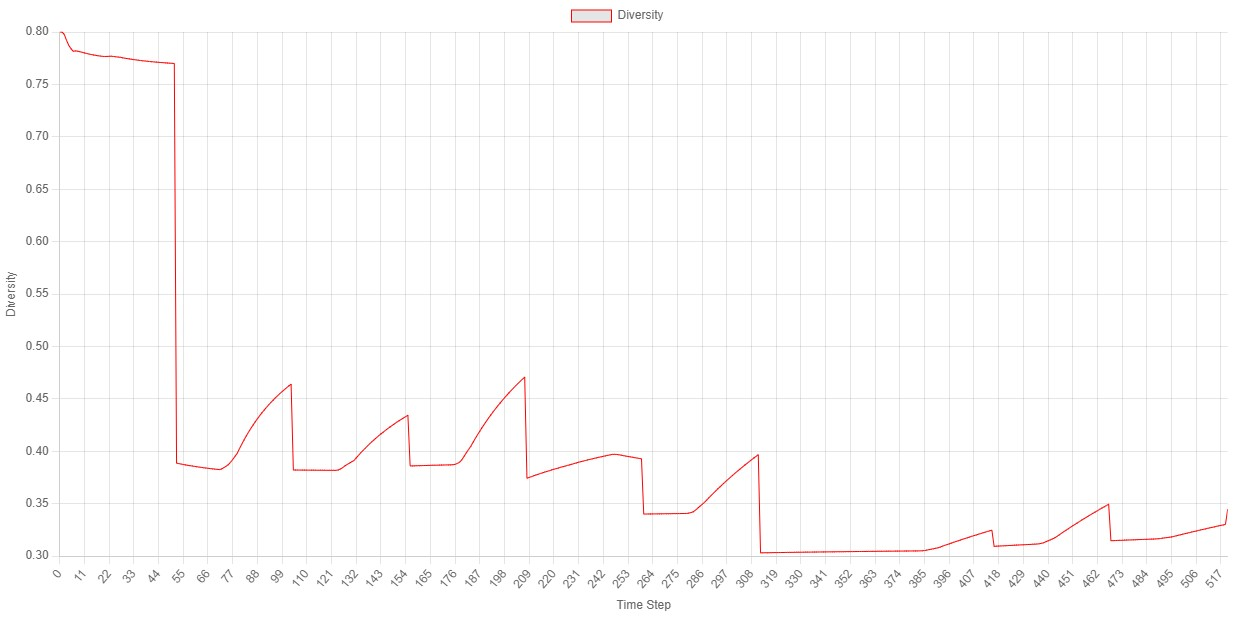
\includegraphics[width=\textwidth]{fig/moderate_chart_diversity.jpg}
    \end{subfigure}
        \begin{subfigure}{0.35\textwidth}
        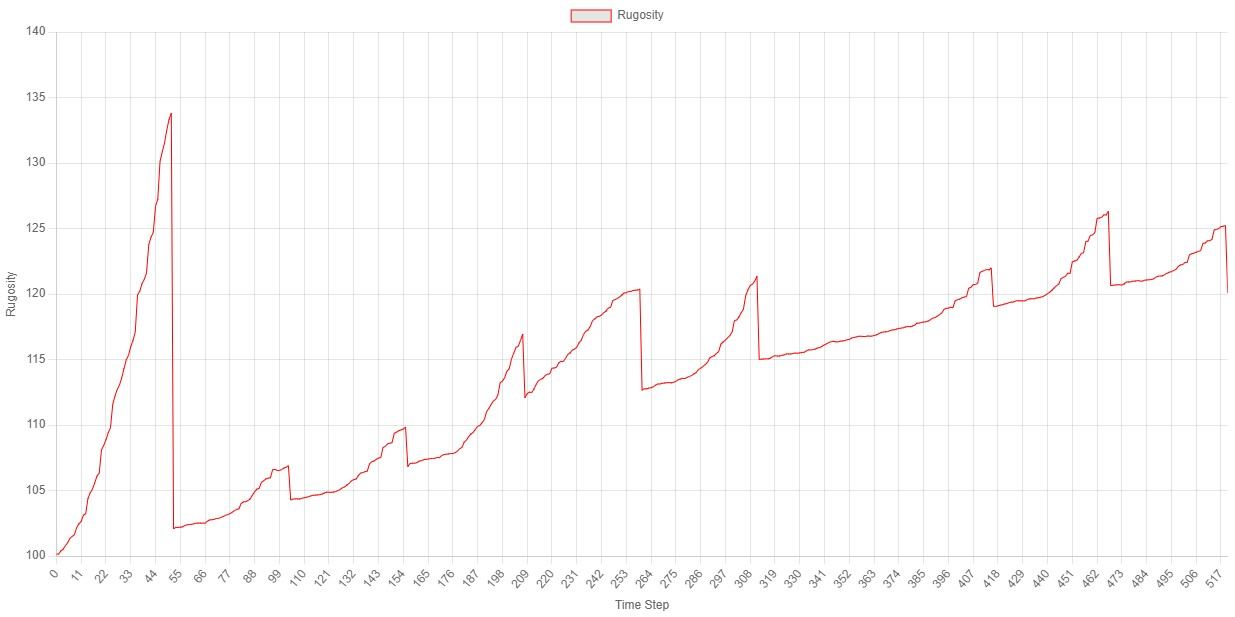
\includegraphics[width=\textwidth]{fig/moderate_chart_rugosity.jpg}
    \end{subfigure}
        \begin{subfigure}{0.25\textwidth}
        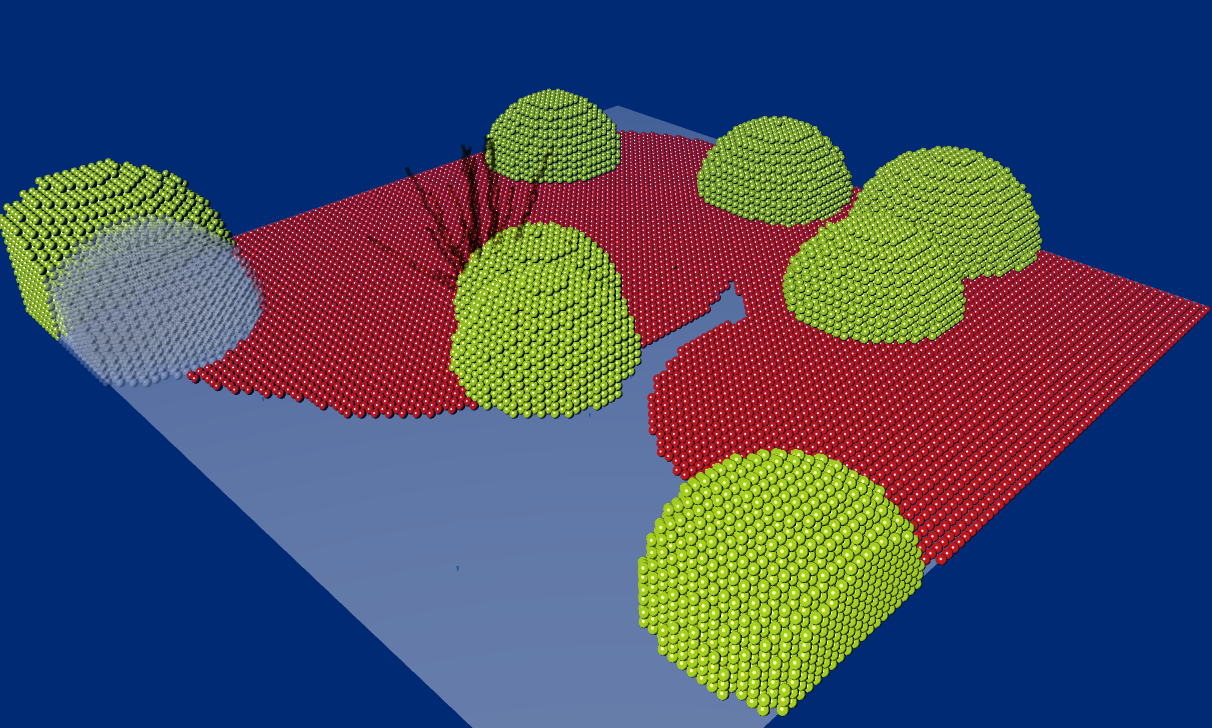
\includegraphics[width=\textwidth]{fig/moderate_visual.png}
    \end{subfigure}
    \caption{Showing results (from left to right and from up down) of flat cover, volume cover, diversity, linear rugosity, and visualisation for moderate occasional disturbance.}
    \label{fig:moderate}
\end{figure}

\begin{figure}[H]
    \centering
    \begin{subfigure}{0.35\textwidth}
        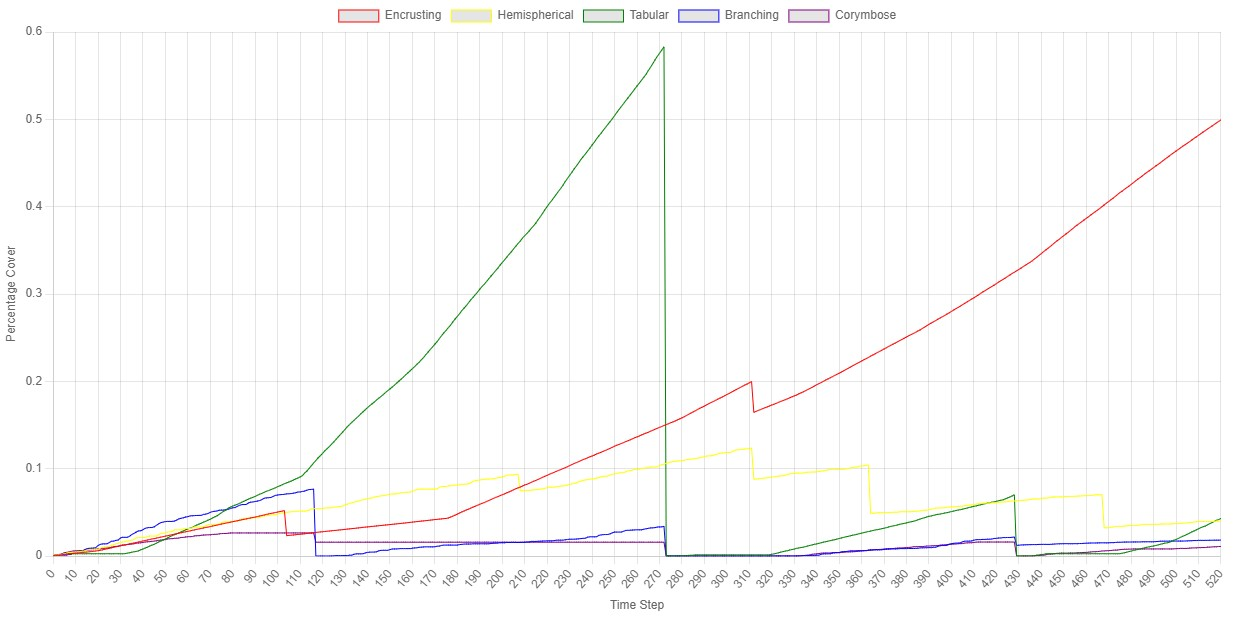
\includegraphics[width=\textwidth]{fig/low_chart_cover.jpg}
    \end{subfigure}
        \begin{subfigure}{0.35\textwidth}
        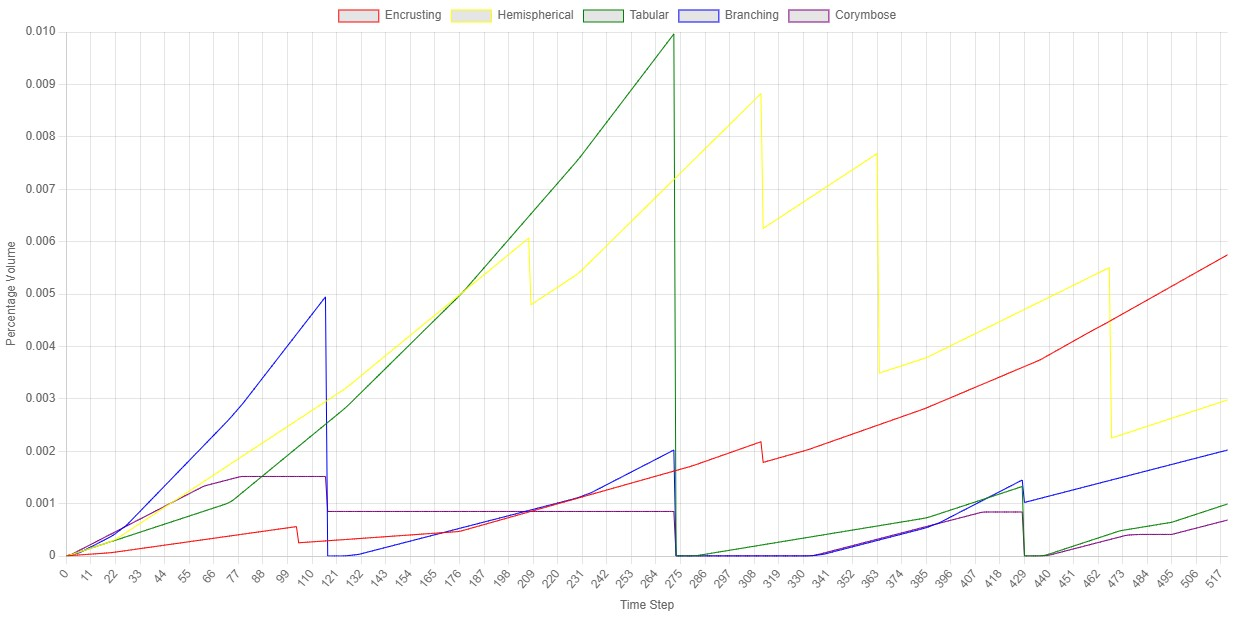
\includegraphics[width=\textwidth]{fig/low_chart_volume.jpg}
    \end{subfigure}
        \begin{subfigure}{0.35\textwidth}
        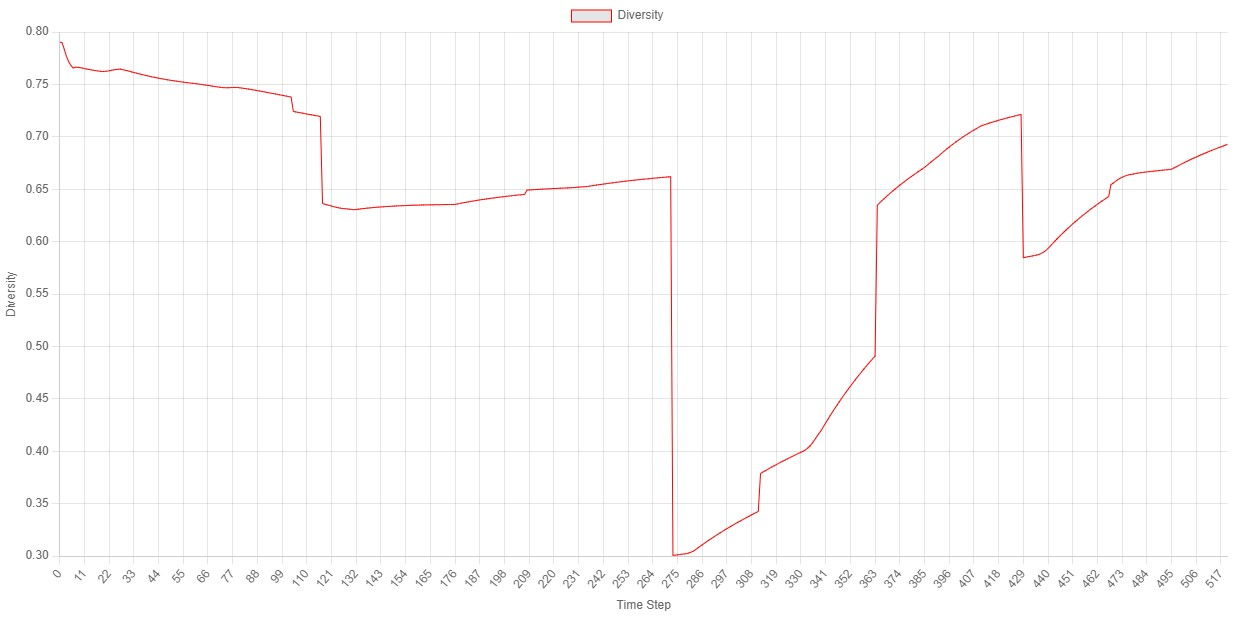
\includegraphics[width=\textwidth]{fig/low_chart_diversity.jpg}
    \end{subfigure}
        \begin{subfigure}{0.35\textwidth}
        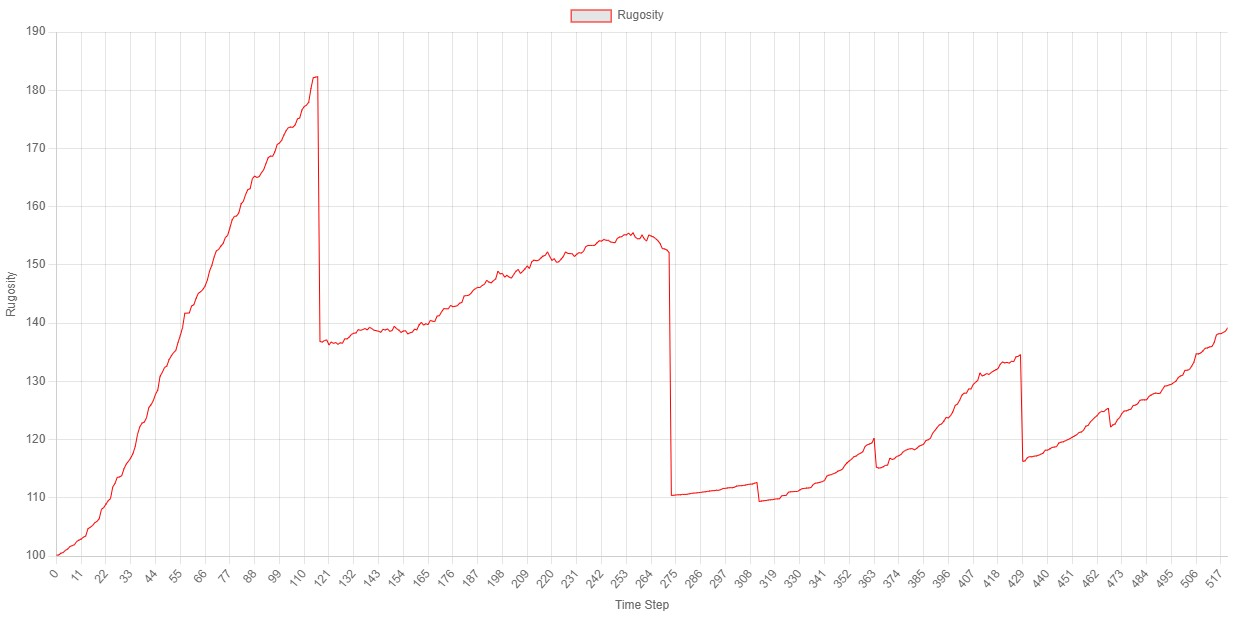
\includegraphics[width=\textwidth]{fig/low_chart_rugosity.jpg}
    \end{subfigure}
        \begin{subfigure}{0.25\textwidth}
        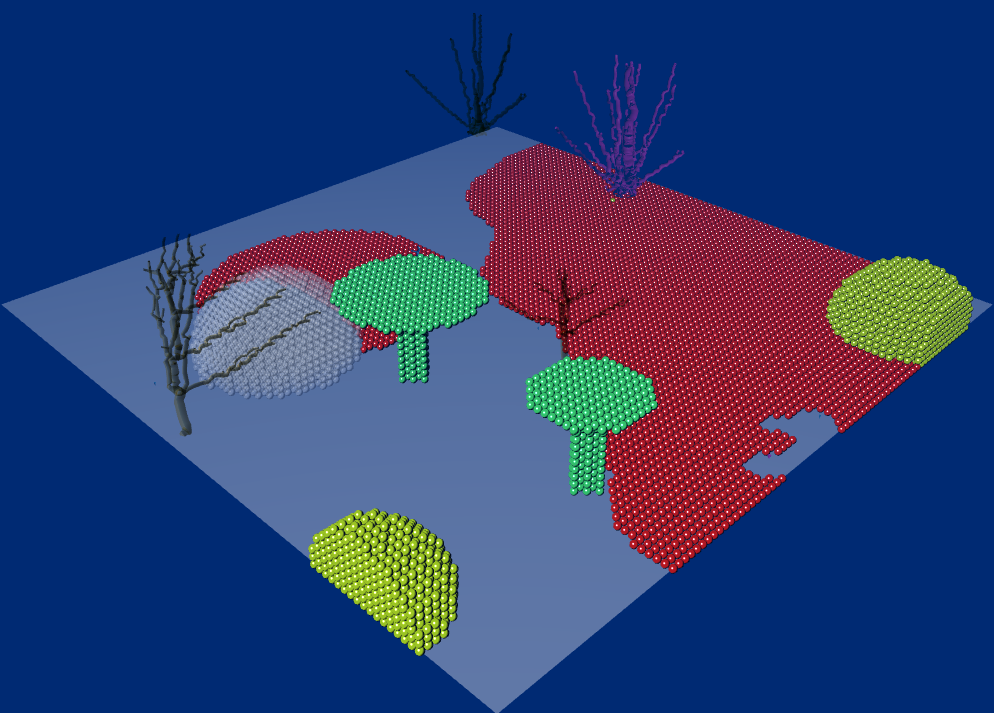
\includegraphics[width=\textwidth]{fig/low_final.png}
    \end{subfigure}
    \caption{Showing results (from left to right and from up down) of flat cover, volume cover, diversity, linear rugosity, and visualisation for common low disturbance.}
    \label{fig:low_common}
\end{figure}

In Figure~\ref{fig:low_common} we can see that even low common disturbances, lead to lower levels of diversity, but through time we can see the reef rebuilding itself, as seen when diversity increases again at the end of the 10 year simulation.

Lastly, we compare the visual results of our model in Figure~\ref{fig:compare}, to the initial \textit{Coralcraft} model, which shows poorer variability and realism of branching and corymbose coral species.

\begin{figure}[H]
    \centering
    \begin{subfigure}{0.35\textwidth}
        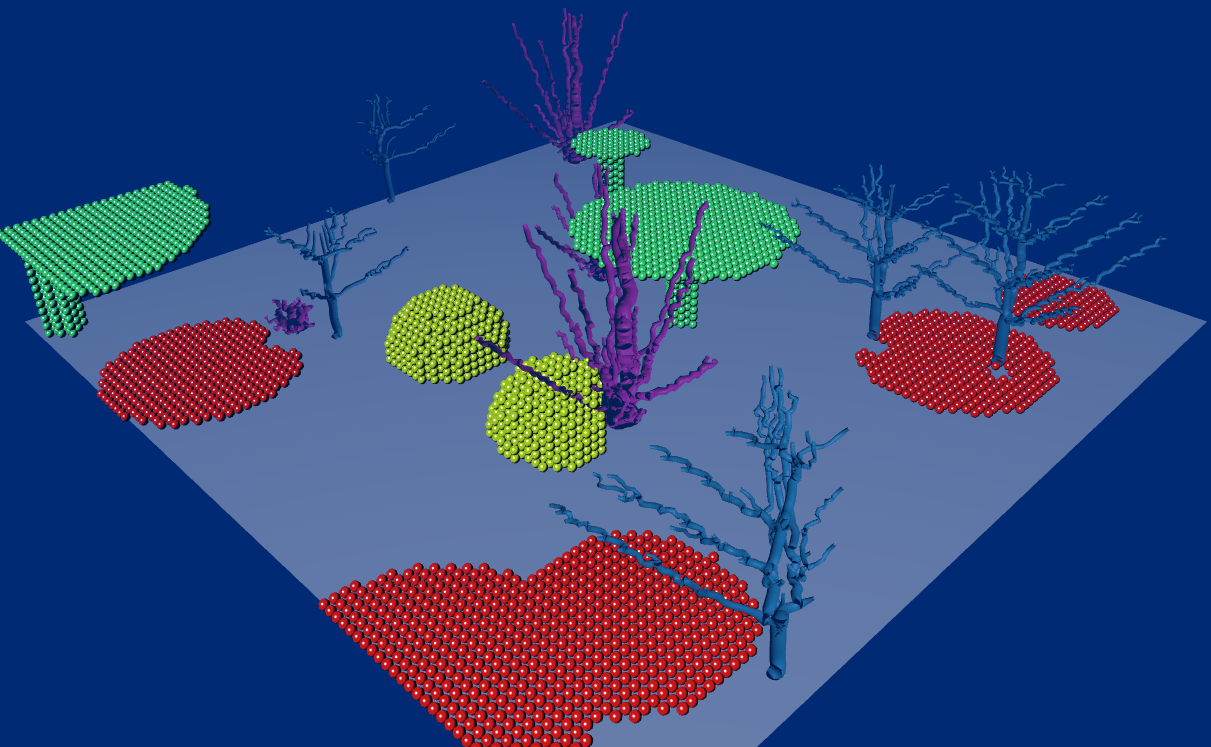
\includegraphics[width=\textwidth]{fig/my_result.png}
    \end{subfigure}
    \begin{subfigure}{0.35\textwidth}
        \includegraphics[width=\textwidth]{fig/Coralcraft.png}
    \end{subfigure}
    \caption{Results of 2 years of simulation between our model on the left and \textit{Coralcraft} model on the right.}
    \label{fig:compare}
\end{figure}

\section*{Discussion}

We optimized the \textit{Coralcraft} model for real-time use. The model reacted to hydrodynamic disturbances as expected, based on the original paper. The reef declined in rugosity and diversity under moderate or high disturbances, leading to reef death in the long run. With low disturbances the diversity also dropped through the simulation, but the reef managed to recover. This matched the original paper and real coral data, but would have to be studied further with a more complex growth model.

The space colonization algorithm enhanced the branching corals’ appearance and diversity, but sea current simulations could improve it more. They affect polyp size and growth direction. Our basic version conflicted with the initial growth model. This was due to the \textit{Coralcraft}’s simple resource simulation based only on light distribution, and would be significantly improved with a fluid simulation and nutrient filtration submodel, but at significant cost to performance.

The initial implementation of the model was very poorly optimized, consuming a lot of memory and computational resources. Therefore, we had to improve both the simulation and rendering process to achieve better performance. For the simulation process, we used more dedicated classes to track intermediary results instead of duplicating large three-dimensional matrices, for each variable of the cellular automata. For the rendering process, we relied on GPU instancing, which can render large numbers of identical meshes in one draw call, reducing the overhead and improving the frame rate. By using these techniques, we were able to create a real-time optimized version of the \textit{Coralcraft} model.

We focused on optimizing and rendering the original \textit{Coralcraft} implementation, which was a challenging and rewarding task. We also explored the possibility of using accretive growth for a more realistic growth model, but we found that the current web technologies do not support the fluid simulation solvers that are required for this approach. We also experimented with WebGPU compute shaders to improve the performance of the simulation, but discovered that the initial model’s light distribution method could not be computed in parallel. Therefore, we decided to use the space colonization algorithm for the growth model.

The implementation of a real-time web version of the model with improved visuals, user interface, and growth model was a successful outcome of this project. We believe that our work contributes to the advancement of coral reef modeling and visualization.

% \pnasbreak splits and balances the columns before the references.
% If you see unexpected formatting errors, try commenting out this line
% as it can run into problems with floats and footnotes on the final page.
%\pnasbreak

\begin{multicols}{2}
\section*{\bibname}
% Bibliography
\bibliography{./bib/bibliography}
\end{multicols}

\end{document}